%!TEX root = ./sujet-projet.tex

\chapter{Analyse du domaine}
\section{Introduction}

Dans ce chapitre, nous présentons l'ensemble des cas d'utilisation que nous avons dégagés lors de l'analyse du domaine. Nous utiliserons pour cela le canevas proposé par Cockburn~\cite{Cockburn:2000} que nous compléterons par des instantanés ainsi que par des post-conditions exprimées en OCL (Object Constraint Language) et quelques scenarii. Cette partie constitue une étape clé de la phase de spécification des besoins. 

Nous présentons également le diagramme des classes métiers (i.e., le diagramme de classes au niveau analyse) que nous avons construit à partir de l'analyse réalisée jusqu'à présent. 
Ce diagramme fournit une vue statique et synthétique du domaine ``\projet'' de notre application. 
Cette dernière partie constitue également une étape clé de la phase de spécification des besoins.


\section{Définition des cas d'utilisation}
Dans cette section, nous spécifions  l'ensemble des cas d'utilisation relatifs au domaine ``\projet''. Le diagramme présenté dans la Figure~\ref{fig:usecases} résume l'ensemble des cas d'utilisation associés de notre système. Ceux-ci peuvent être effectués par deux acteurs différents:
 \begin{itemize}
 \item Le chef de département;
 \item l'enseignant.
 \end{itemize}

 \vspace{2cm}

 \begin{figure}[!htbp]
 \begin{center}
 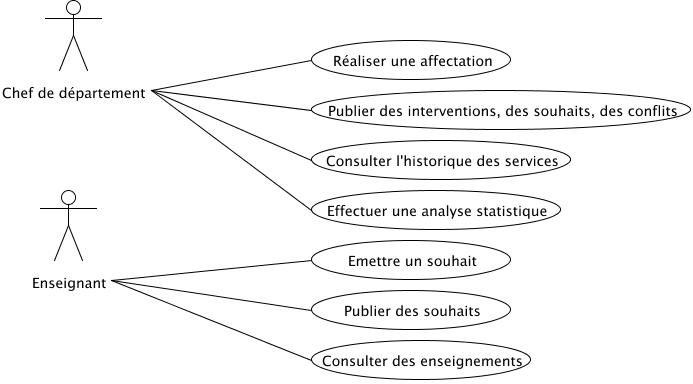
\includegraphics[width=14cm]{fig/useCaseDiagram.jpg}
 \caption{Cas d'utilisation du domaine "\projet".}
 \end{center}
 \label{fig:usecases}
 \end{figure}

Dans les sections suivantes, nous fournissons une description plus détaillée de chacun des cas d'utilisation.

\subsection{UC1 - Réaliser une affectation}

\begin{usecase}{Réaliser une affectation}
	\begin{information}

 \item[Goal in the context:] Le chef de département réalise la confirmation d'un souhait d'un enseignant (validation) ou impose une intervention dans le département à un enseignant (affectation ``forcée''). 
 L'enseignant devra se soumettre aux décisions du chef de département que ce soit pour une validation d'un souhait ou une affectation imposée.

\item[Scope:] Département

 \item[{Level:}]
 Résumé

 \item[{Precondition:}]
 Le chef de département connait pour l'enseignant concerné : les souhaits (seulement ceux déjà publiés par l'enseignant), les possibles conflits et les affectations le concernant.

 \item[{Success End Condition:}]
 L'enseignant est affecté à un ou plusieurs enseignements (souhait validé ou intervention imposée). Le volume horaire total effectué par l'enseignant a été recalculé.

 \item[{Failed End Condition:}]
 L'affectation n'a pas été réalisée (l'enseignement est déjà affecté à un autre enseignant : conflit).

 \item[Primary actor:]
 Chef de département.

 \item[Trigger:]
 Demande de réalisation d'une affectation faite par le chef de département.\\

\end{information}
 %\\
% \noindent\textbf{MAIN SUCCESS SCENARIO}
 \begin{scenario}
 \item Le chef de département demande au système de visualiser l'ensemble des souhaits des enseignants.
 \item Le système renvoie les souhaits qui ont été publiés par les enseignants.
 \item Le chef de département sélectionne des souhaits, selon certains critères (l'enseignant, le module concerné, \dots).
 \item Le système renvoie les souhaits correspondants aux critères.  
 \item Le chef de département choisit un v\oe u d'un enseignant afin de le valider.
 \item Le système valide le v\oe u, l'enseignement associé au v\oe u est affecté à l'enseignant concerné : c'est-à-dire que le v\oe u donne lieu à une intervention effective.\\
 \end{scenario}

 %\\
% \noindent\textbf{EXTENSIONS}
 \begin{extension}
 \item [5a] Le chef de département choisit d'imposer une intervention à un enseignant dans son département (affectation imposée).
 \item [5a1] Le système affecte l'intervention à l'enseignant.
 \item [5b] L'utilisateur choisit de valider une demande d'intervention extérieure ou une demande spéciale (remplacement, encadrement de stage, congés, \dots) de l'enseignant.
 \item [5b1] Le système affecte l'intervention ou valide la demande spéciale de l'enseignant sans créer de conflits avec les autres enseignants.\\
 \end{extension}
\end{usecase}

 \subsubsection{Instantané: réaliser une affectation}
 \indent Cas d'utilisation : \textbf{Réaliser une affectation} - Acteur : \textbf{Chef de département}.
 \begin{figure}[!htbp]
 \begin{center}
 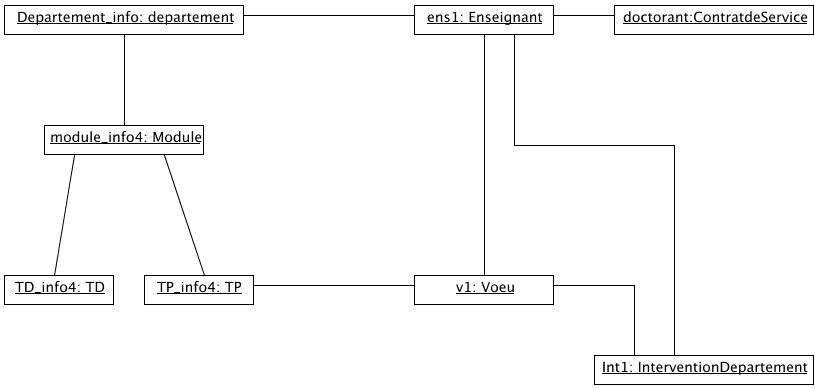
\includegraphics[width=12cm]{fig/3-RealisationVoeu.jpg}
 \caption{Réalisation d'une affectation à partir d'un v\oe u}
 \end{center}
 \end{figure}

 \indent La réalisation d'une affectation à partir d'un v\oe u par un chef de département crée une instance de la classe \textbf{InterventionDépartement}. Celle-ci est associée au v\oe u validé et, par conséquent, à l'enseignement concerné.

 \begin{ocl}
 context Departement::realiserVoeu(v : Voeu)
 post : not v.peut_donner_lieu_a.isUndefined()
        and v.emet.est_affecte_pour -> include(v.peut_donner_lieu_a)
 \end{ocl}
 
 \emph{Le v\oe u réalisé donne lieu à une InterventionDepartement qui fait parti de la liste d'affectation de l'enseignant (celui qui a émis ce v\oe u : v.emet). Cette réalisation est effectuée par le chef de département.}


 \subsubsection{Instantané: réaliser une affectation à partir d'une demande extérieure}
 \indent  Cas d'utilisation : \textbf{Réaliser une affectation} - Acteur : \textbf{Chef de département}.
 \begin{figure}[!htbp]
 \begin{center}
 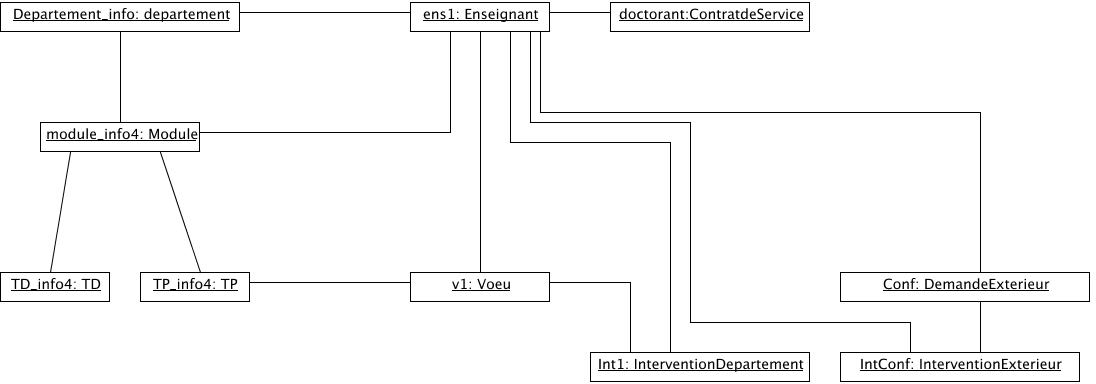
\includegraphics[width=14cm]{fig/6-RealisationDemandeExterieur.jpg}
 \caption{Réalisation d'une affectation à partir d'une demande extérieure}
 \end{center}
 \end{figure}

 \indent La réalisation d'une affectation à partir d'une demande extérieure crée une nouvelle instance de la classe \textbf{InterventionExtérieure} associée à la demande extérieure et à l'enseignant concerné.

 \begin{verbatim}
 context Departement::realiserDemandeExterieure(de : DemandeExterieure)
 post : not de.peut_donner_lieu.isUndefined()
        and de.emet.est_affecte_pour -> include(de.peut_donner_lieu)
 \end{verbatim}
 \emph{La DemandeExterieure réalisée donne lieu à une InterventionExterieure qui fait parti de la liste d'affectation de l'enseignant (celui qui a émis cete DeamdeExterieure : de.emet). Cette réalisation est effectuée par le chef de département.}


 \subsubsection{Instantané: réaliser une affectation à partir d'une demande spéciale}
 \indent Cas d'utilisation : \textbf{Réaliser une affectation} - Acteur : \textbf{Chef de département}

 \begin{figure}[!htbp]
 \begin{center}
 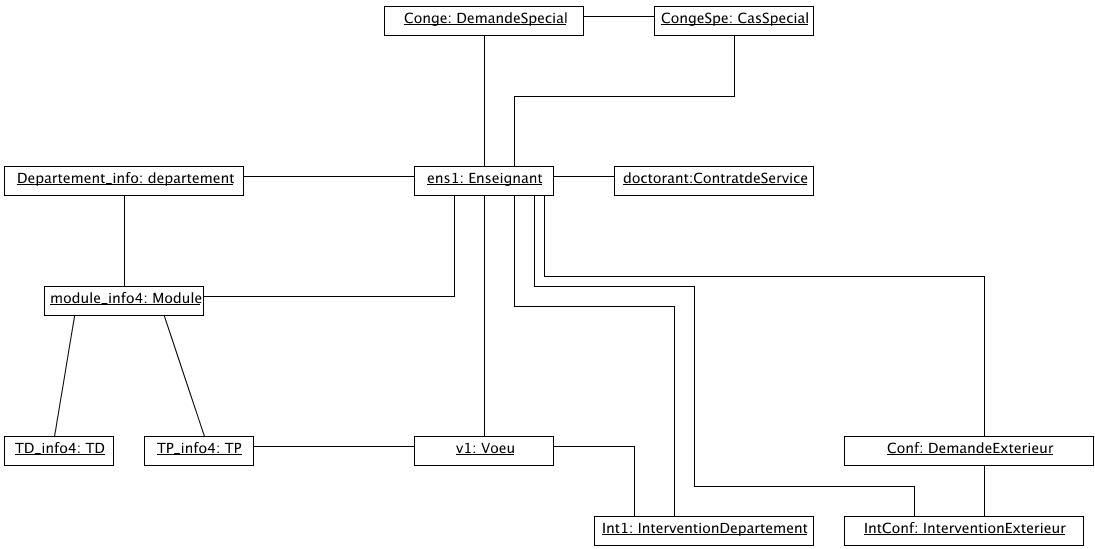
\includegraphics[width=14cm]{fig/8-RealisationSpecial.jpg}
 \caption{Réalisation d'une affectation à partir d'une demande spéciale}
 \end{center}
 \end{figure}

 \indent La réalisation d'une affectation d'une demande spéciale crée l'instance de la classe \textbf{CasSpécial} associé à l'enseignant et à la demande spéciale concernés.

 \begin{ocl}
 context Departement::realiserDemandeSpeciale(ds : DemandeSpeciale)
 post : not ds.peut_donner_lieu.isUndefined()
        and ds.emet.est_affecte_pour -> include(ds)
 \end{ocl}
 
 \emph{La DemandeSpeciale réalisée donne lieu à un CasSpecial qui fait parti de la liste d'affectation de l'enseignant (celui qui a émis cete DemandeSpeciale : de.emet). Cette réalisation est effectuée par le chef de département.}

 \subsubsection{Instantané: imposer une intervention dans le département à un enseignant}
 \indent Cas d'utilisation : \textbf{Réaliser une affectation} - Acteur : \textbf{Chef de département}

 \begin{figure}[!htbp]
 \begin{center}
 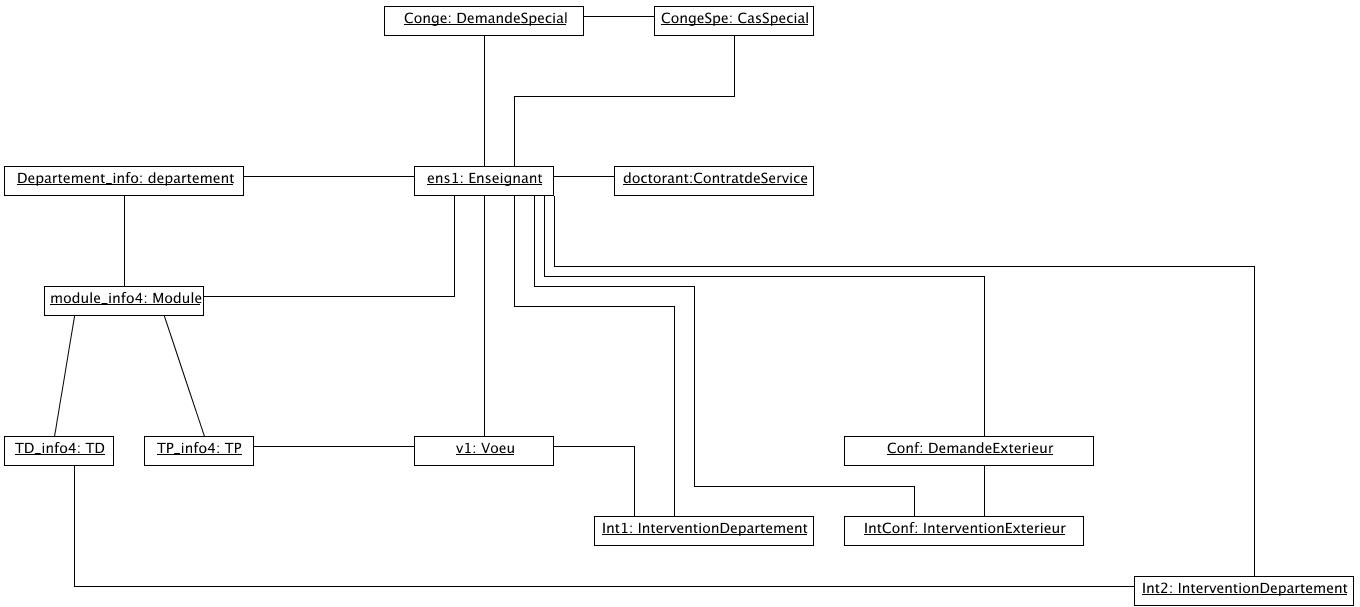
\includegraphics[width=14cm]{fig/9-ImpositionVoeu.jpg}
 \caption{Imposition d'une intervention dans le département à un enseignant}
 \end{center}
 \end{figure}

 \indent L'imposition d'une intervention à un enseignant crée une instance de la classe \textbf{InterventionDepartement} associée à l'enseignant et à l'enseignement concernés. Les interventions (dans le département) imposées ne sont pas liées à un v\oe u.

 \begin{ocl}
 context Departement::imposeInterventionDepartement(ens : Enseignant, e : Enseignement)
 post : not e.interventiondepartement.isUndefined()
        and ens.est_affecte_pour -> include(e.interventionDepartement)
 \end{ocl}
 
 \emph{L'enseignement e est lié à une unique InterventionDepartement qui appartient à la liste des affectations de l'enseignant ens. C'est le chef de département qui impose cette InterventionDepartement.}


 \subsubsection{Instantané: imposition d'une intervention à un enseignant par le chef de département}
 \begin{figure}[!htbp]
 \begin{center}
 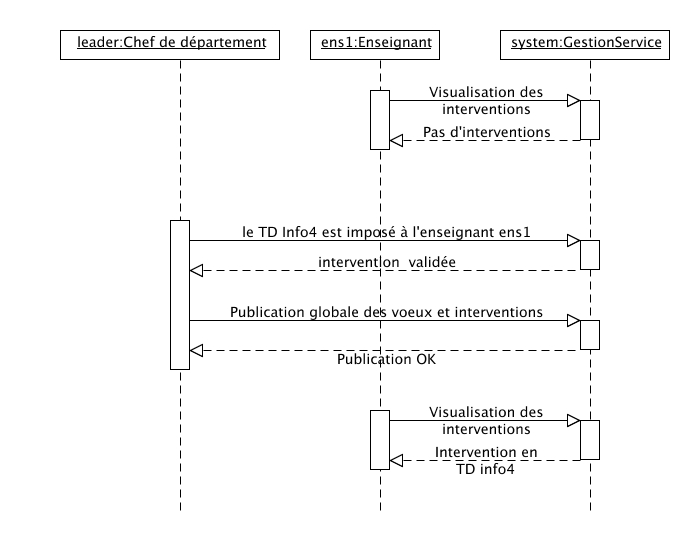
\includegraphics[width=15cm]{fig/scenario3.jpg}
 \caption{Scénario : imposition d'une intervention à un enseignant par le chef de département}
 \end{center}
 \end{figure}

 Dans ce scénario, le chef de département impose une intervention concernant un enseignement de son département. L'affectation est donc imposée à l'enseignant.  

 \subsubsection{Instantané: imposer une affectation de type ``cas spécial'' (ex : arrêt maladie)}
 \indent Cas d'utilisation : \textbf{Réaliser une affectation} - Acteur : \textbf{Chef de département}

 \begin{figure}[!htbp]
 \begin{center}
 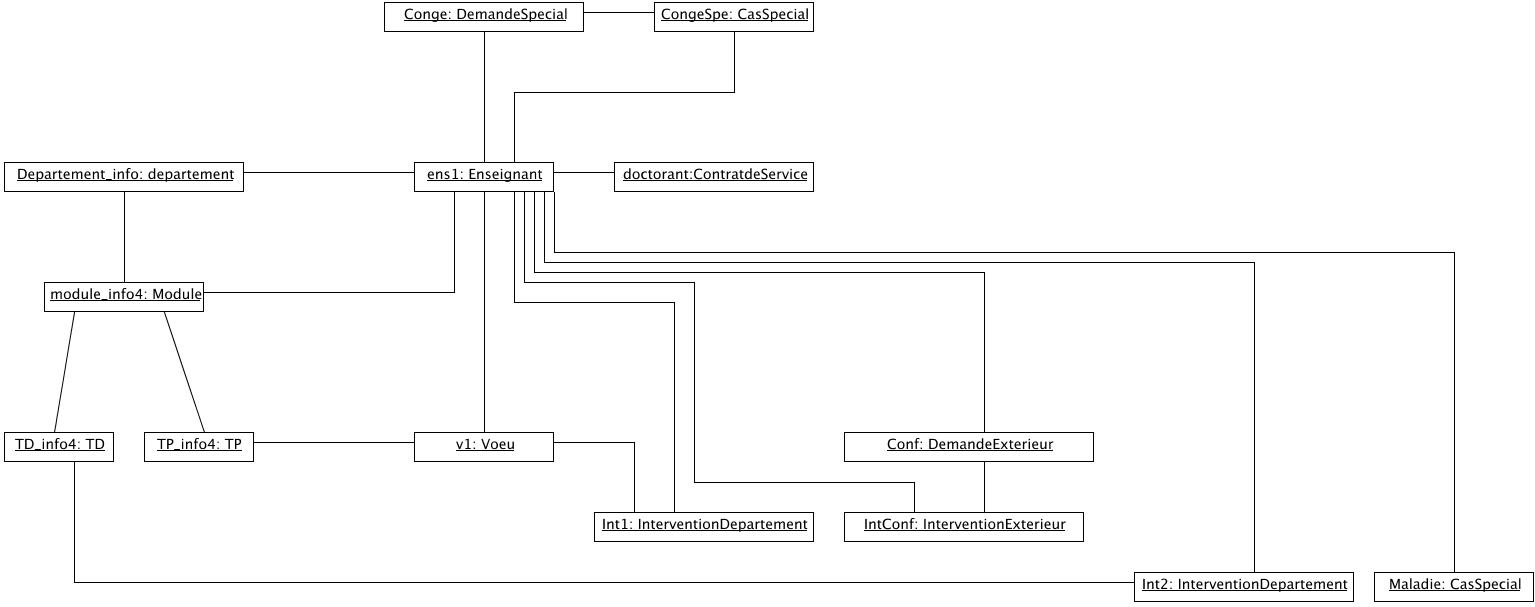
\includegraphics[width=14cm]{fig/10-ImpositionCasSpecial.jpg}
 \caption{Imposer une affectation de type ``cas spécial'' (ex : arrêt maladie)}
 \end{center}
 \end{figure}

 \indent L'imposition d'une affectation de type ``cas spécial'' à un enseignant crée une instance de la classe \textbf{CasSpécial} associée à l'enseignant concerné. Ce ``cas spécial'' n'est pas lié à une demande spéciale (puisqu'elle a été imposée).

 \begin{verbatim}
 context Departement::imposeCasSpecial(ens : Enseignant, c : CasSpecial)
 post : ens.est_affecte_pour -> include(c)
 \end{verbatim}
 \emph{Le CasSpecial c, appartient à la liste des affectations de l'enseignant ens. C'est le chef de département qui impose ce CasSpecial.}


%Afin d'avoir une vue plus globale de l'application, nous avons rédigé quelques scénarii faisant intervenir différents acteurs et différents cas d'utilisation. Ces scénarii sont exprimés sous la forme de diagrammes de séquence.

 \subsubsection{Conflit entre deux enseignants - résolution par le chef de département}
 \begin{figure}[!htbp]
 \begin{center}
 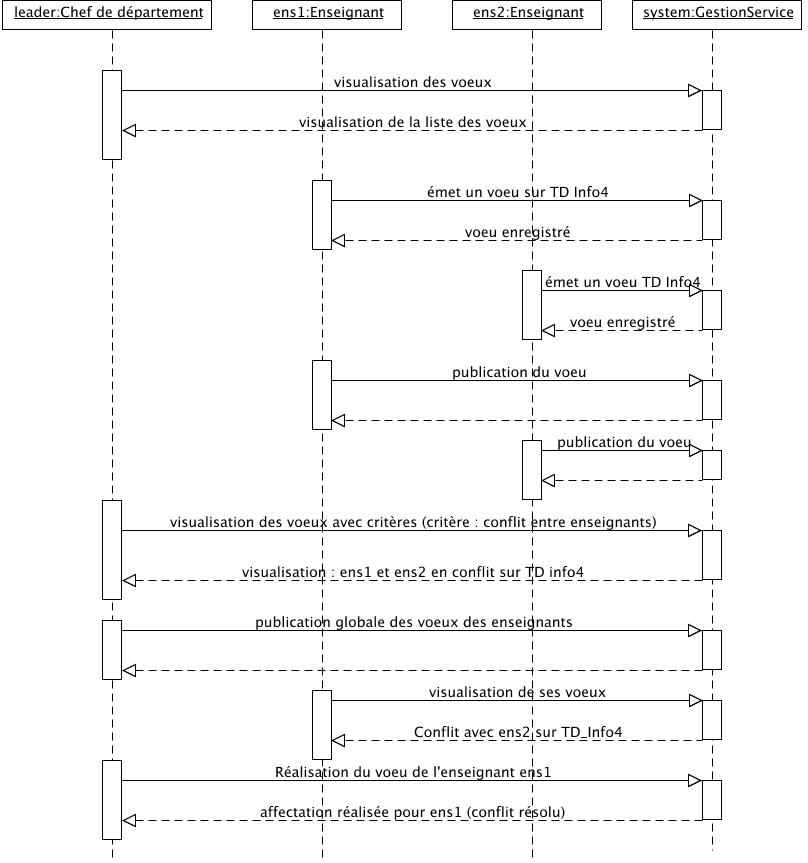
\includegraphics[width=15cm]{fig/scenario1.jpg}
 \caption{Scénario : conflit entre deux enseignants - résolution par le chef de département}
 \end{center}
 \end{figure}

 Dans ce scénario, le conflit est réglé par le chef de département qui affecte l'enseignement à un seul des deux enseignants (la demande de l'autre enseignant est alors considérée comme étant refusée).

 \subsubsection{Conflit entre deux enseignants - résolution par un des enseignants}
 \begin{figure}[!htbp]
 \begin{center}
 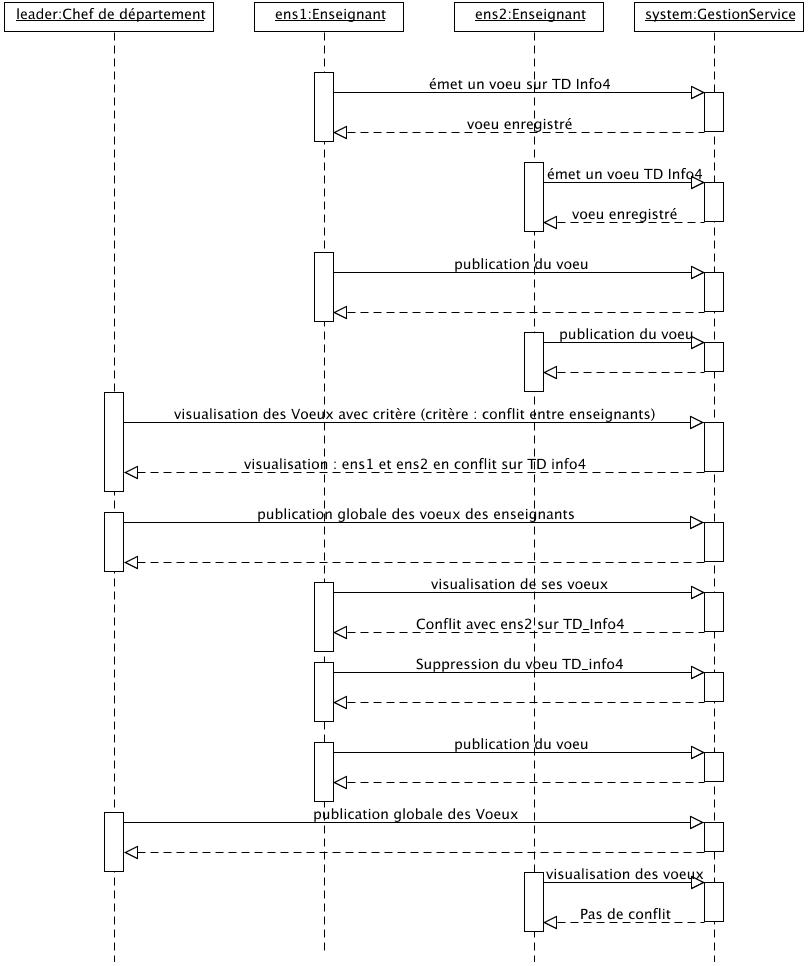
\includegraphics[width=15cm]{fig/scenario2.jpg}
 \caption{Scénario : conflit entre deux enseignants - résolution par un des enseignants}
 \end{center}
 \end{figure}

 Dans ce scénario, le conflit est réglé par un des deux enseignants qui annule son v\oe u concernant l'enseignement à l'origine du conflit.  


\subsection{UC2 - Publier des interventions, des souhaits et des possibles conflits}

 \noindent\textbf{Use Case:} 2 - Publier des interventions, des souhaits et des possibles conflits

 \noindent\--------------------------------------

 \noindent\textbf{CHARACTERISTIC INFORMATION}\\

 \noindent \textbf{Goal in the context:}
 Le chef de département, par cette action, permet aux autres acteurs du système (en l'occurence les enseignants) de visualiser les informations concernant l'état actuel des souhaits et des affectations (interventions) de l'ensemble des enseignants. L'exécution de ce cas d'utilisation peut faire apparaître de nouveaux conflits pour les enseignants.

 \noindent\textbf{Scope:}
 Département

 \noindent\textbf{Level:}
 Résumé

 \noindent\textbf{Precondition:}
 \

 \noindent\textbf{Success End Condition:}
 Les enseignants ont accès aux informations concernant l'état actuel des souhaits et des affectations publiés. Dans le cas de publication d'interventions, le volume horaire des enseignants concernés est recalculé. Des conflits peuvent apparaître localement pour chaque enseignant.

 \noindent\textbf{Failed End Condition:}
 Echec de la publication : les enseignants n'ont toujours pas accès aux informations que le chef de département a tenté de publier.

 \noindent\textbf{Primary actor:}
 Chef de département.

 \noindent\textbf{Trigger:}
 Demande de publication des interventions, des souhaits et des conflits possibles faite par le chef de département.\\

 %\\
 \noindent\textbf{MAIN SUCCESS SCENARIO}
 \begin{enumerate}
 \item Le chef de département visualise l'ensemble des souhaits et des affectations non publiés.
 \item L'application renvoie l'ensemble des information voulues.
 \item L'utilisateur sélectionne un ensemble de souhait et d'affectations.
 \item Le systeme les rend publics pour les autres enseignants.\\
 \end{enumerate}

 %\\
 \noindent\textbf{EXTENSIONS}
 \begin{list}{}{}
 \item Pas d'extensions\\
 \end{list}


 \subsection{UC3 - Consulter l'historique des services suivant différents critères}

 \noindent\textbf{Use Case:} 3 - Consulter l'historique des services suivant différents critères

 \noindent\--------------------------------------

 \noindent\textbf{CHARACTERISTIC INFORMATION}\\

 \noindent \textbf{Goal in the context:}
 Le chef de département visualise les affectations (interventions) et les souhaits par rapport à une année donnée. Le tri ou la sélection peut se faire selon les critères suivants :
 \begin{itemize}
 \item Par module et enseignement ;
 \item par enseignant ;
 \item par nombre d'heures effectives et/ou souhaitées.
 \end{itemize}

 \noindent\textbf{Scope:}
 Département

 \noindent\textbf{Level:}
 Résumé

 \noindent\textbf{Precondition:}
 Les années demandées sont antérieures ou égales à l'année actuelle.

 \noindent\textbf{Success End Condition:}
 Le chef de département visualise les informations demandées.

 \noindent\textbf{Failed End Condition:}
 L'année n'existe pas dans l'historique du système (aucune entrée disponible pour les critères demandés).

 \noindent\textbf{Primary actor:}
 Chef de département.

 \noindent\textbf{Trigger:}
 Demande de consultation de l'historique des services faite par le chef de département.\\

 
 %\\
 \noindent\textbf{MAIN SUCCESS SCENARIO}
 \begin{enumerate}
 \item Le chef de département décide de visualiser l'ensemble des souhaits et des interventions d'une année donnée selon ses critères.
 \item Le système renvoie l'ensemble des souhaits et des interventions correspondants aux critères demandés.\\
 \end{enumerate}

 %\\
 \noindent\textbf{EXTENSIONS}
 \begin{list}{}{}
 \item 2a. Le système ne renvoie rien puisqu'aucune entrée n'existe dans l'historique pour cette année.\\
 \end{list}



 \subsection{UC4 - Effectuer une analyse statistique}

 \noindent\textbf{Use Case:} 4 - Effectuer une analyse statistique 

 \noindent\--------------------------------------

 \noindent\textbf{CHARACTERISTIC INFORMATION}\\

 \noindent \textbf{Goal in the context:}
 Le chef de département effectue une analyse statistique permettant de déterminer la répartition des volumes horaires par enseignants ou la répartition des souhaits et affectations entre enseignants pour une année donnée. Ce cas d'utilisation étend le cas d'utilisation numéro 3.

 \noindent\textbf{Scope:}
 Département

 \noindent\textbf{Level:}
 Résumé

 \noindent\textbf{Precondition:}
 /

 \noindent\textbf{Success End Condition:}
 L'utilisateur visualise le résultat de l'étude statistique.

 \noindent\textbf{Failed End Condition:}
 /

 \noindent\textbf{Primary actor:}
 Chef de département.

 \noindent\textbf{Trigger:}
 Demande de réalisation d'un analyse statistique faite par le chef de département.\\

 %\\
 \noindent\textbf{MAIN SUCCESS SCENARIO}
 \begin{enumerate}
 \item Le chef département sélectionne les données qu'il désire ``analyser''. (cas d'utilisation n°3)
 \item Le chef de département choisit le type d'analyse statistique qu'il souhaite effectuer.
 \item Le système renvoie le résultat de l'analyse.\\
 \end{enumerate}

 %\\
 \noindent\textbf{EXTENSIONS}
 \begin{list}{}{}
 \item Pas d'extensions\\
 \end{list}


 \subsection{UC5 - Émettre un souhait}

 \noindent\textbf{Use Case:} 5 - \'Emettre un souhait

 \noindent\--------------------------------------

 \noindent\textbf{CHARACTERISTIC INFORMATION}\\

 \noindent \textbf{Goal in the context:}
 L'enseignant émet un souhait. Le souhait correspond à v\oe u sur un ensemble d'enseignements (avec une préférence) du département, une demande d'intervention extérieure au département ou une demande spéciale (arrêt maladie, remplacement,\dots)

 \noindent\textbf{Scope:}
 Département

 \noindent\textbf{Level:}
 Résumé

 \noindent\textbf{Precondition:}
 En cas de v\oe ux sur des enseignements, ces derniers doivent exister et être non affectés à un autre enseignant.

 \noindent\textbf{Success End Condition:}
 Le souhait de l'enseignant a été pris en compte par le système mais n'est pas encore publié c'est-à-dire que seul l'enseignat peut le voir (i.e. cette modification est locale). Localement, le volume horaire total (le volume horaire effectif plus la somme des volumes horaires des souhaits pas encore validés) de l'enseignant est modifié (recalculé) par rapport au volume horaire précisé dans le souhait.

 \noindent\textbf{Failed End Condition:}
 Dans le cas d'un v\oe u, l'enseignement a déjà été affecté ou n'existe plus.

 \noindent\textbf{Primary actor:}
 Enseignant.

 \noindent\textbf{Trigger:}
 Demande d'émission d'un souhait faite par l'enseignant.\\

 %\\
 \noindent\textbf{MAIN SUCCESS SCENARIO}
 \begin{enumerate}
 \item L'enseignant décide de visualiser l'ensemble des enseignements disponibles (i.e. non affectés) dans son département (cas d'utilisation n°7).
 \item Le système lui renvoie la liste de ces enseignements.
 \item L'enseignant fait son choix en sélectionnant un ensemble d'enseignements, indique son niveau de préférence pour ces enseignements (voulus ou seulement souhaités) et valide.
 \item Le systeme enregistre localement ce souhait.\\
 \end{enumerate}

 %\\
 \noindent\textbf{EXTENSIONS}
 \begin{list}{}{}
 \item 1a. L'enseignant décide de faire une demande concernant une intervention extérieure au département, précise le volume horaires, l'organisme concerné et valide son choix.
 \item 1b. L'enseignant décide de faire une demande spéciale souhaité en précisant le type (un congé, un remplacement, \dots), le volume horaire et valide son choix.
 \item 4a. Le v\oe u génère un conflit (avec d'autres souhaits déjà rendus publics) : le système le notifie à l'enseignant.
 \item 4b. Le souhait génère un surplus d'heures pour l'enseignant (par rapport à son contrat de services) : le système le notifie à l'enseignant.\\
 \end{list}

 \subsubsection{Instantané: émettre un souhait}
 \indent Cas d'utilisation : \textbf{\'Emettre un souhait} - Acteur : \textbf{Enseignant}.

 \begin{figure}[!htbp]
 \begin{center}
 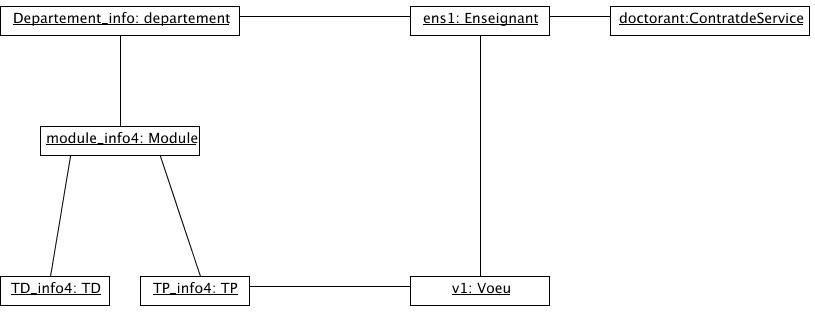
\includegraphics[width=12cm]{fig/2-emissionVoeu.jpg}
 \caption{\'Emission d'un v\oe u}
 \end{center}
 \end{figure}

 \indent L'émission d'un v\oe u provoque l'ajout d'une instance de la classe \textbf{V\oe u} à l'enseignant associé et concernant l'enseignement demandé. Dans ce cas, nous avons défini une demande de v\oe u simple (demande d'un v\oe u sur un seul enseignement).

 \begin{ocl}
 context Enseignant::emettreVoeu(v : Voeu)
 post : self.emet -> include(v)
        and not v.concerne -> isEmpty()
 // le voeu ajouté appartient à la liste des voeux de l'enseignant et concerne au moins un enseignement
 \end{ocl}
 \emph{Le v\oe u ajouté appartient à la liste des souhaits (self.emet) de l'enseignant et concerne au moins un enseignement. C'est l'enseignant qui ajoute ce v\oe u à sa liste de souhaits.}

 \subsubsection{Instantané: émettre une demande extérieure}
 \indent Cas d'utilisation : \textbf{\'Emettre un souhait} - Acteur : \textbf{Enseignant}.

 \begin{figure}[!htbp]
 \begin{center}
 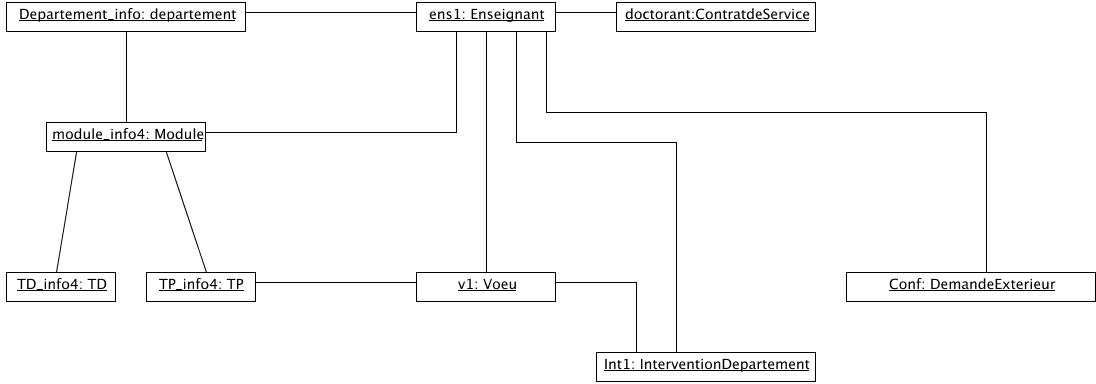
\includegraphics[width=14cm]{fig/5-EmissionDemandeExterieur.jpg}
 \caption{\'Emission d'une demande extérieure}
 \end{center}
 \end{figure}

 \indent L'émission d'une demande extérieure crée une nouvelle demande extérieure associée à l'enseignant.
 \begin{verbatim}
 context Enseignant::emettreDemandeExterieure(d : DemandeExterieure)
 post : self.emet -> include(d)
 \end{verbatim}
 \emph{La DemandeExterieure ajoutée appartient à la liste des souhaits (self.emet) de l'enseignant. C'est l'enseignant qui ajoute cette DemandeExterieure à sa liste de souhaits.}

 \subsubsection{Instantané: émettre une demande spéciale}
 \indent Cas d'utilisation : \textbf{\'Emettre un souhait} - Acteur : \textbf{Enseignant}.

 \begin{figure}[!htbp]
 \begin{center}
 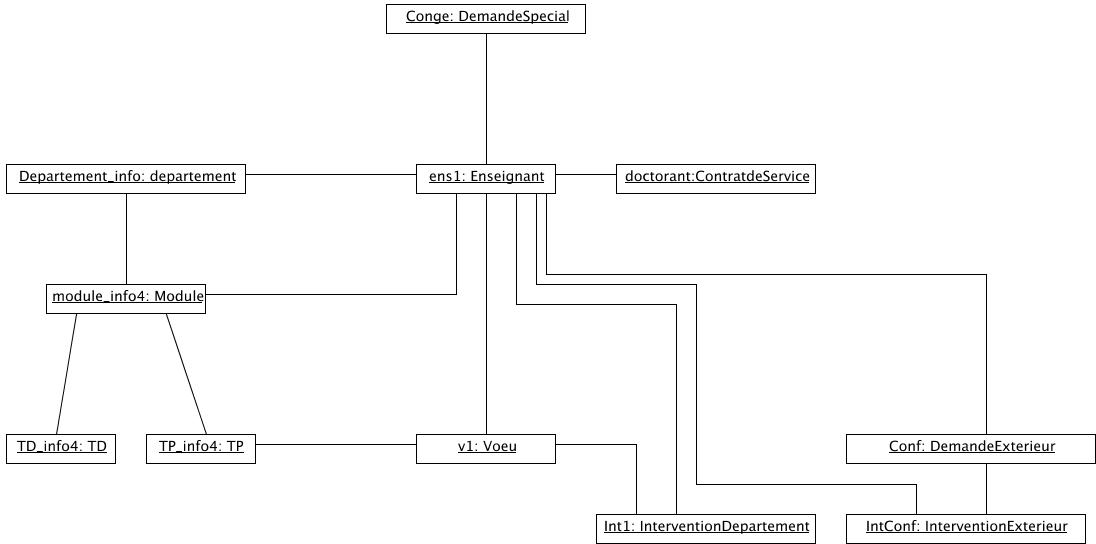
\includegraphics[width=14cm]{fig/7-EmissionSpecial.jpg}
 \caption{\'Emission d'une demande spéciale}
 \end{center}
 \end{figure}

 \indent L'émission d'une demande spéciale crée la demande spéciale associée à l'enseignant.

 \begin{ocl}
 context Enseignant::emettreDemandeSpeciale(ds : DemandeSpeciale)
 post : self.est_affecte_pour -> include(ds)
 \end{ocl}
 \emph{La DemandeSpeciale ajoutée appartient à la liste des souhaits (self.emet) de l'enseignant. C'est l'enseignant qui ajoute cette DemandeSpeciale à sa liste de souhaits.}



 \subsection{UC6 - Publier des souhaits}

 \noindent\textbf{Use Case:} 6 - Publier des souhaits

 \noindent\--------------------------------------

 \noindent\textbf{CHARACTERISTIC INFORMATION}\\

 \noindent \textbf{Goal in the context:}
 L'utilisateur transmet ses souhaits (préalablement sélectionnés) au chef de département qui sera lui même apte, dans un deuxième temps, à les rendre visibles à l'ensemble des enseignants (cas d'utilisation n°2).
 Un souhait concerne un vœux fait sur des enseignements disponibles (i.e. non affectés), une intervention extérieure au département ou bien encore une demande caractérisée comme étant spéciale (congé, remplacement, \dots). 


 \noindent\textbf{Scope:}
 Département

 \noindent\textbf{Level:}
 Résumé

 \noindent\textbf{Precondition:}
 Le/les souhaits concernés ont été préalablement réalisés et validés localement par l'enseignant.

 \noindent\textbf{Success End Condition:}
 Le chef de département est capable de visualiser le/les souhaits publiés par l'enseignant.

 \noindent\textbf{Failed End Condition:}
 Le souhait concerne un enseignement qui a déjà été affecté entre temps par le chef de département.

 \noindent\textbf{Primary actor:}
 Enseignant.

 \noindent\textbf{Trigger:}
 Demande de publication de souhaits faite par l'enseignant.\\
 
 %\\
 \noindent\textbf{MAIN SUCCESS SCENARIO}
 \begin{enumerate}
 \item L'enseignant choisit de visualiser l'ensemble des souhaits qu'il a réalisé localement mais qu'il n'a pas encore publié. (cas d'utilisation n°5)
 \item Le système lui renvoie l'ensemble de ces souhaits classés selon leur type (i.e. v\oe u, intervention extérieure et demande spéciale)
 \item L'utilisateur choisit, parmi ces souhaits, ceux qu'il désire publier.
 \item Le système enregistre la publication et transmet les souhaits au chef de département.\\
 \end{enumerate}

 %\\
 \noindent\textbf{EXTENSIONS}
 \begin{list}{}{}
 \item 2a. Le système lui signifie qu'il n'existe pas de souhaits qui sont en attente d'être publiés.
 \item 3a. L'enseignant décide de ne publier aucun de ces souhaits et annule sa demande de publication.
 \item 4a. Le système signifie à l'utilisateur que l'un de ces souhaits (en l'occurence un v\oe u) concerne un ou plusieurs enseignements qui ont été affectés ou supprimés et lui demande de modifier son v\oe u (cas d'utilisation n°5).\\
 \end{list}


 \subsection{UC7 - Consulter des enseignements suivant différents critères}

 \noindent\textbf{Use Case:} 7 - Consulter des enseignements suivant différents critères

 \noindent\--------------------------------------

 \noindent\textbf{CHARACTERISTIC INFORMATION}\\

 \noindent \textbf{Goal in the context:}
 L'enseignant doit être capable de visualiser les enseignements afin de consulter ou de modifier ses souhaits.
 Ainsi, des critères de tri sont mis à sa disposition pour personnaliser sa vue des enseignements dans le système ``Gestion de services''.
 Voici une liste de ces critères :
 \begin{itemize}
 \item Par module ;
 \item par enseignement d'un module ;
 \item par enseignant ;
 \item par nombre d'heures.
 \end{itemize}

 De plus, il doit choisir les critères de sélection des enseignements qu'il souhaite visualiser:
 \begin{itemize}
 \item Les enseignements concernés par des v\oe ux publiés ou non ;
 \item les enseignements concernés par des v\oe ux déjà validés (affectations) ;
 \item les enseignements affectés et ceux non affectés.
 \end{itemize}

 L'enseignant peut choisir de visualiser les enseignements des années précédentes mais il ne pourra effectuer aucune modification sur ces années. Par défaut, la visualisation se fera sur l'année en cours.

 L'utilisateur choisit l'ensemble des critères de tri et de sélection sur les enseignements qu'il souhaite. Il peut donc entièrement paramétrer sa vue des enseignements.

 \noindent\textbf{Scope:}
 Département

 \noindent\textbf{Level:}
 Résumé

 \noindent\textbf{Precondition:}

 \noindent\textbf{Success End Condition:}

 \noindent\textbf{Failed End Condition:}

 \noindent\textbf{Primary actor:}
 Enseignant.

 \noindent\textbf{Trigger:}
 Demande de consultation des enseignements selon différents critères faite par l'enseignant.

 %\\
 \noindent\textbf{MAIN SUCCESS SCENARIO}
 \begin{enumerate}
 \item L'enseignant décide de visualiser l'ensemble des enseignements selon ses critères.
 \item Le système renvoie l'ensemble des enseignements correspondants aux critères demandés.\\
 \end{enumerate}

 %\\
 \noindent\textbf{EXTENSIONS}
 \begin{list}{}{}
 \item 2a. Le système ne renvoie rien puisqu'aucun enseignement ne correspond aux critères demandés.
 \end{list}



 %*********
 \subsection{Instantanés et contraintes OCL sur les cas d'utilisation}
 \indent Nous allons vous présenter, dans cette sous-partie, un ensemble représentatif d'instantanés des cas d'utilisation. Nous allons donc partir d'un système vide (seul le département est représenté avec un module et deux enseignements) pour ensuite illustrer l'évolution de notre système au cours de son utilisation.\\
 \indent Voici le diagramme d'instances qui va nous servir de point de départ pour nos instantanés (nous considérons comme triviale la création des modules et des enseignements associés à un département) :

 \begin{figure}[!htbp]
 \begin{center}
 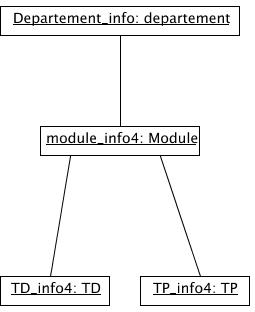
\includegraphics[width=4cm]{fig/base.jpg}
 \caption{Instantané de départ}
 \end{center}
 \end{figure}

 \subsubsection{Assigner un enseignant à un département}
 \indent Cas d'utilisation : non mentionné car basique - Acteur : \textbf{Chef de département}.

 \begin{figure}[!htbp]
 \begin{center}
 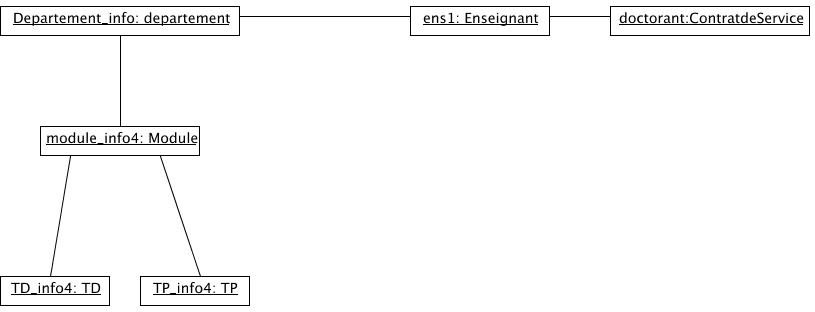
\includegraphics[width=12cm]{fig/1-assignEnseignant.jpg}
 \caption{Assignation d'un enseignant}
 \end{center}
 \end{figure}

 \indent L'assignation d'un nouvel enseignant au département provoque l'ajout d'une instance de la classe \textbf{Enseignant} ainsi que du contrat de service qui lui est associé (instance de la classe \textbf{ContratDeService}).

 \begin{verbatim}
 context Departement::assignerEnseignant(e : Enseignant)
 post : self.enseignant.include(e)
        and not e.contratdeservice.isUndefined()
 \end{verbatim}
 \emph{L'enseignant appartient au département et possède un contrat de service unique. L'assignation provient du chef de département.}







 \subsubsection{Assigner un responsable à un module}
 \indent Cas d'utilisation : \textbf{Assigner un responsable} - Acteur : \textbf{Chef de département}.

 \begin{figure}[!htbp]
 \begin{center}
 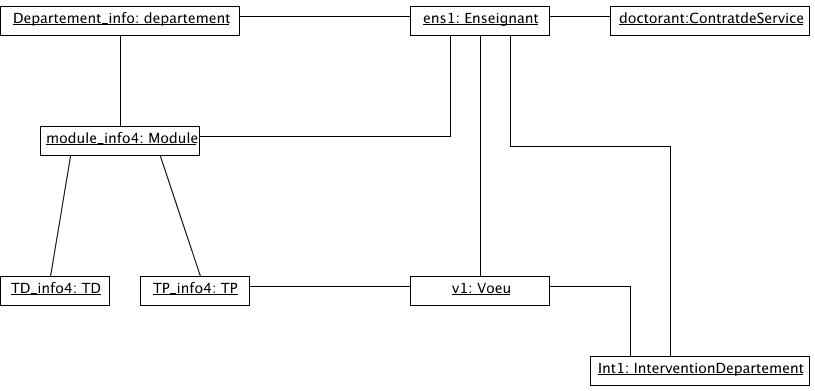
\includegraphics[width=12cm]{fig/4-ResponsableModule.jpg}
 \caption{Assignation d'un responsable à un module}
 \end{center}
 \end{figure}

 \indent L'assignation d'un responsable de module associe un enseignant au module dont il devient le responsable.

 \begin{verbatim}
 context Departement::assignerResponsable(m : Module, ens : Enseignant)
 post : m.est_responsable_de = ens
 \end{verbatim}
 \emph{L'enseignant ens devient responsable du module m. Cette assignation est réalisée par le chef de département}


 \section{Diagramme de classes métiers}
Afin d'achever cette phase de spécification des besoins, nous fournissons une modélisation statique et synthétique du domaine de notre application. La figure~\ref{cls-metier} représente ce domaine ``Gestion des services'' : 

 \begin{figure}[!htb]
 \centering
 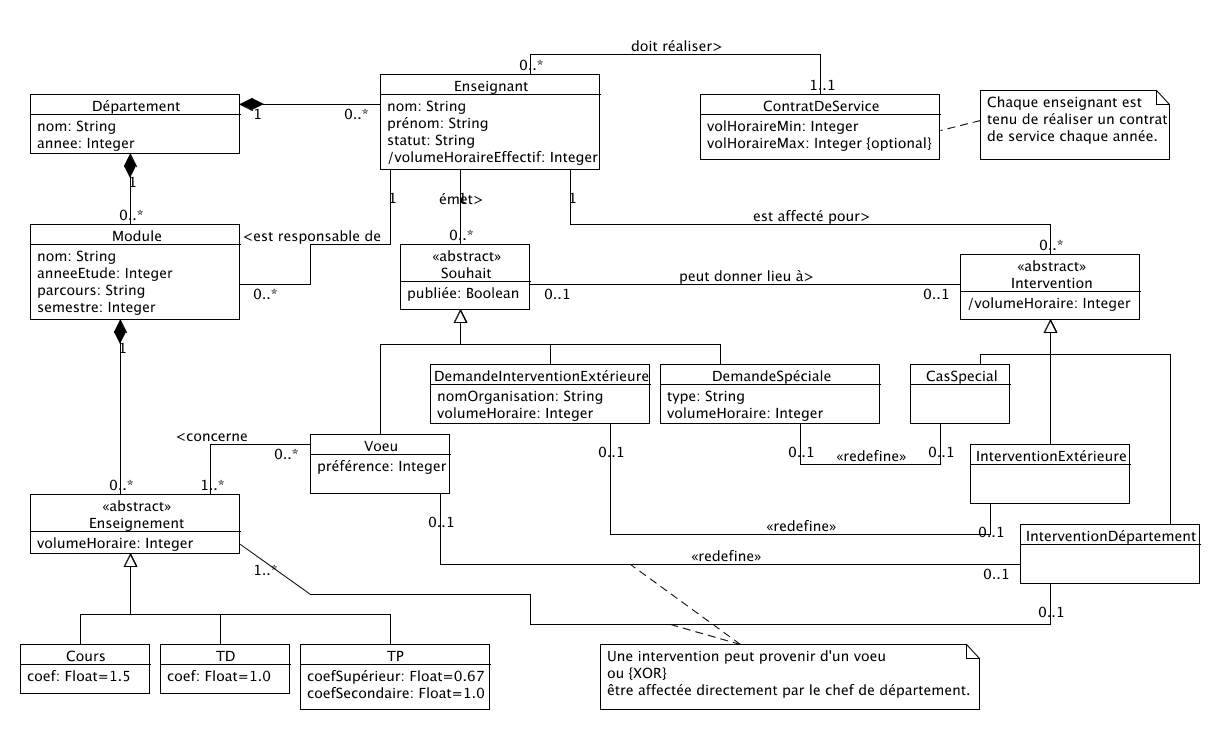
\includegraphics[width=18cm] {fig/ClassesMetiers.jpg}
 \caption{Diagramme de classes métiers du domaine ``Gestion des services''}
 \label{cls-metier}
 \end{figure}

 Le domaine "Gestion des services" est composé d'un ensemble de départements identifiés par leur nom et leur année (ex : département ``Informatique, 2004'', département ``Informatique, 2005'', département ``Mathématiques, 2005'', \dots). Chacun de ces départements est constitué de modules et possède un certain nombre d'enseignants qui lui sont rattachés.\\ 

 Un module est défini par un nom, une année d'étude (ex : 2$^{\textrm{\footnotesize{eme}}}$ année), un parcours (ex : ``Licence Informatique'') et un semestre (1$^{\textrm{\footnotesize{er}}}$ ou 2$^{\textrm{\footnotesize{eme}}}$). Il se décompose en plusieurs enseignements avec pour chacun un volume horaire et un coefficient : il peut s'agir de cours magistraux (CM), de travaux dirigés (TD) ou de travaux pratiques (TP). Chaque module a pour responsable un enseignant qui se doit, en principe, d'assurer un certain nombre d'enseignements dans ce module (le plus souvent les cours magistraux).\\

 Les enseignants sont caractérisés par leur nom et leur statut et doivent chacun remplir un contrat de service par année, c'est-à-dire effectuer un certain nombre d'heures minimum d'enseignement par année (calculé à partir des coefficients des enseignements). Il est important de noter que le contrat de service est uniquement fonction du statut de l'enseignant et est indépendant du département auquel il est rattaché.\\

 Chaque enseignant peut émettre un certain nombre de souhaits afin d'indiquer la manière dont il désire remplir son contrat de service. Ces souhaits peuvent être des v\oe ux (indications du ou des enseignements que l'enseignant souhaite dispenser ainsi que ses préférences les concernant), des demandes d'intervention extérieure (dans une entreprise, une autre école...) ou des demandes spéciales (congés, arrêts maladie, encadrements de stages ou de TER\dots).\\ 

 Il est ensuite du ressort du chef du département concerné de décider de valider ou non ces souhaits, i.e. d'affecter ou non à l'enseignant concerné les interventions correspondantes aux souhaits émis. Toutefois, pour régler certains conflits, le chef d'un département se réserve le droit d'imposer une affectation à un enseignant sans que cet enseignant en ait auparavant formulé le souhait.\\ 

 Pour terminer, notons que l'attribut nommé ``année'', présent dans la classe ``Département'', permet d'assurer la persistance des données concernant les modules, les enseignants, les souhaits et les interventions des différents enseignants au fil des années. Ainsi, il sera possible de construire un historique des souhaits et des interventions dans notre système. Cela pourra s'avérer très utile afin de permettre au chef de département de tenir compte des demandes des années passées pour le guider dans ses choix d'affectation concernant l'année en cours. Nous ne nous étendons pas sur le sujet de la persistance puisque ce n'est pas l'objectif de la phase de spécification des besoins. 




 % \section{Conclusion}
 % En produisant ce livrable, nous avons été amené à réaliser la phase de spécification des besoins concernant l'application ``Gestion des services''. Cette phase s'est déroulée en plusieurs étapes. Nous avons tout d'abord étudié le cahier des charges fourni pour élaborer un dictionnaire du domaine ``Gestion des services''. Puis en s'appuyant sur cette analyse, nous avons dégagé l'ensemble des cas d'utilisation de notre système que nous avons par la suite décrits à l'aide du canevas proposé par Cockburn et mis en \oe uvre dans des scénarii. Nous avons également expliçité un certain nombre de contraintes non-fonctionnelles et de plateforme concernant notre application. Enfin, nous avons fourni une vue statique de notre domaine qui se veut à la fois synthétique et complète, i.e. regroupant et articulant l'ensemble des concepts métiers liés à ce domaine.\\
 %
 % Ce premier livrable va servir de point de départ dans le processus de conception de notre application. Nous allons le considérer dans les trois autres livrables (détermination de l'architecture, spécification des composants et conception détaillée) comme étant notre référence, notre base de travail. Cependant, comme dans tout processus d'analyse et de conception, la démarche reste itérative. Ce qui veut dire que ce document fera sûrement l'objet de quelques modifications dans le futur lorsque nous travaillerons sur les autres livrables, l'important étant de fournir au final (au client et aux développeurs) un dossier d'analyse et de conception aussi cohérent qu'abouti.

 %**************************************************************


 % \nocite{*}
 % \bibliography{bib}
 %
 %
 % \end{document}
 
 
 
 
% \section{Introduction}
%
% \subsection{Objectif}
% Décrire l'objectif de ce chapitre.
%
% \subsection{Organisation du chapitre}
% Ce chapitre est organisé en $n$ sections. Dans le première section, nous décrirons....
%
%
%
% \section{Exemple de code OCL}
% \begin{ocl}
% context Etudiant::age() : Integer
% post correct: result = (today - naissance).years()
%
% context Typename::operationName(param1: type1, ...): Type
% post: result = ...
%
% context Typename::operationName(param1: type1, ...): Type
% post resultOk: result = ...
% \end{ocl}
%
% \section{Exemple d'un cas d'utilisation}
%
% \subsection{Réaliser une affectation}
%
% \begin{usecase}{Réaliser une affectation}
%
% \begin{information}
%
% \item[Goal in the context:]
% Le chef de département réalise la confirmation d'un souhait d'un enseignant (validation) ou impose une intervention dans le département à un enseignant (affectation ``forçée''). L'enseignant devra se soumettre aux décisions du chef de département que ce soit pour une validation d'un souhait ou une affectation imposée.
%
% \item[Scope:]
% Département
%
% \item[Level:]
% Résumé
%
% \item[Precondition:]
% Le chef de département connait pour l'enseignant concerné : les souhaits (seulement ceux déjà publiés par l'enseignant), les possibles conflits et les affectations le concernant.
%
% \item[Success End Condition:]
% L'enseignant est affecté à un ou plusieurs enseignements (souhait validé ou intervention imposée). Le volume horaire total effectué par l'enseignant a été recalculé.
%
% \item[Failed End Condition:]
% L'affectation n'a pas été réalisée (l'enseignement est déjà affecté à un autre enseignant : conflit).
%
% \item[Primary actor:]
% Chef de département.
%
% \item[Trigger:]
% Demande de réalisation d'une affectation faite par le chef de département.\\
%
% \end{information}
%
% %\\
% \begin{scenario}
% \item Le chef de département demande au système de visualiser l'ensemble des souhaits des enseignants.
% \item Le système renvoie les souhaits qui ont été publiés par les enseignants.
% \item Le chef de département sélectionne des souhaits, selon certains critères (l'enseignant, le module concerné, \dots).
% \item Le système renvoie les souhaits correspondants aux critères.
% \item Le chef de département choisit un v\oe u d'un enseignant afin de le valider.
% \item Le système valide le v\oe u, l'enseignement associé au v\oe u est affecté à l'enseignant concerné : c'est-à-dire que le v\oe u donne lieu à une intervention effective.\\
% \end{scenario}
%
% %\\
% \begin{extension}
% \item[5a] Le chef de département choisit d'imposer une intervention à un enseignant dans son département (affectation imposée).
% \item[5a1] Le système affecte l'intervention à l'enseignant.
% \item[5b] L'utilisateur choisit de valider une demande d'intervention extérieure ou une demande spéciale (remplacement, encadrement de stage, congés, \dots) de l'enseignant.
% \item[5b1] Le système affecte l'intervention ou valide la demande spéciale de l'enseignant sans créer de conflits avec les autres enseignants.\\
% \end{extension}
% \end{usecase}
%
%
% \section{Conclusion}
%
